\subsection{ДЕТАЛЬНОЕ ОБСУЖДЕНИЕ И ОБЪЯСНЕНИЕ ФИЗИЧЕСКИХ МЕХАНИЗМОВ}\label{subsec:2-6}

Была обнаружена связь КМД с ИП в том числе и в результатах моделирования ГЭЦ. Используя данные вкладов одиночных столбцов модели возможно проанализировать найденную связь более детально. В данном подразделе будет предпринята попытка разложить вариацию ИП на простые колебания, чтобы понять физический механизм, лежащий за наблюдаемым эффектом.

В климатологии принято вычислять ЭОФ и ГК для различных физических параметров с целью идентифицировать КМД \cite{Knutson_Weickmann_1987, Slingo_et_al_1999, Lo_Hendon_2000, Matthews_2000, Kessler_2001}. ЭОФ являются определёнными собственными векторами данных, которые отражают основные пространственные паттерны, в то время как ГК являются зависящими от времени коэффициентами разложения исходных данных по базису, составленному из ЭОФ. В разделе \ref{sec:rmm} было описано, как в \cite{Wheeler_Hendon_2004} используют ЭОФ и ГК (рассчитанные для комбинированного набора данных, составленного из зональных ветров на двух высотах и OLR), чтобы ввести индекс RMM, который используется для описания КМД. В данном разделе будет применён ЭОФ-анализ к моделируемым вкладам в ИП, это позволит свести сложную изменчивость ИП к нескольким простым осцилляциям, имеющим понятный физический смысл и легко интерпретируемым в терминах КМД.

\subsubsection{ПРЕДВАРИТЕЛЬНАЯ ОБРАБОТКА ВКЛАДОВ В ИП}
\label{sec:preliminary_processing}

Как и в \cite{Wheeler_Hendon_2004} рассматривался приэкваториальный регион, ограниченный с севера и с юга широтами 15\textdegree~с.~ш. и 15\textdegree~ю.~ш. соответственно. Согласно результатам моделирования ГЭЦ в среднем данный регион даёт 86\% от всего ИП, что делает данный регион ключевым в изучении связи ГЭЦ с КМД. Моделируемые вклады в ИП суммировались вдоль каждой из 360 полосок 1\textdegree\texttimes30\textdegree около экватора (15\textdegree~с.~ш. -- 15\textdegree~ю.~ш. по широте и 0\textdegree~--~1\textdegree~в.~д., 1\textdegree~в.~д.~--~2\textdegree~в.~д. и так далее до 1\textdegree~з.~д. -- 0\textdegree\ по долготе), в результате чего получался один набор данных длиной 360 для каждого моделируемого дня. Такое суммирование упрощает сложный процесс эволюции вкладов в ИП в течение цикла КМД путём вычитания меридиональной структуры, которая показана на рис. \ref{fig:map_of_contributions}. Так как первостепенным в КМД является процесс переноса с запада на восток конвективной структуры, то в первом приближении можно рассматривать лишь долготную структуру вкладов для изучения связей ГЭЦ с КМД.

КМД всегда случается совместно с прочей конвективной изменчивостью, поэтому важно некоторым образом выявить во вкладах в ИП и удалить большую часть изменчивости, не связанной с КМД. Похожий подход применялся и в \cite{Wheeler_Hendon_2004} до расчета ЭОФ.

Прежде всего удалялась связь ГЭЦ с ЭНЮК \cite{Harrison_et_al_2011, Slyunyaev_et_al_2021c}. Для этих целей вычислялся коэффициент линейной регрессии между средними за день значениями вкладов в ИП от приэкваториальных полос 1\textdegree\texttimes30\textdegree\ на разной долготе и температурой поверхности океана (ТПО), усреднённая по региону Niño 3.4 (5\textdegree\ с. ш. -- 5\textdegree\ ю. ш. и 120\textdegree\ в. д. -- 170\textdegree\ в. д.), который хорошо характеризует ЭНЮК. Из каждой полосы 1\textdegree\texttimes30\textdegree\ вычиталась найденная линейная связь с ТПО региона Niño 3.4, при этом сохранялось долговременное среднее значение (точнее из вкладов в ИП вычитались значения, предсказанные линейной аппроксимацией на основе ТПО региона Niño 3.4 в соответствующие дни, при этом регулировался постоянный член этой линейной аппроксимации таким образом, чтобы среднее значение вклада данной полосы 1\textdegree\texttimes30\textdegree, вычисленное за 41 год моделирования, не изменилось).

После этого из вкладов удалялась сезонная вариация \cite{Adlerman_Williams_1996}. Для этого было применено дискретное преобразование Фурье к временному ряду вкладов каждой из полос 1\textdegree\texttimes30\textdegree, значения Фурье-спектра, отвечающие первым четырём гармоникам сезонного цикла, (то есть те, которые соответствовали периоду $T=365.25\, \textnormal{дней}$, $T/2$, $T/3$ и $T/4$) клались равными нулю, затем производилось обратное дискретное преобразование Фурье. Стоит отметить, что данную  операцию следует проводить после удаления связи с вкладов с ЭНЮК, ведь ТПО региона Niño 3.4 имеет свои собственные сезонные гармоники, поэтому вычитание из вкладов величин пропорциональных ТПО региона Niño 3.4 приводит к усилению сезонных гармоник вкладов в ИП. Кроме того, следует отметить, что вычитание сезонных гармоник не изменяет среднее значение, так как долговременное среднее значение каждой гармоники равно нулю.

Рис. \ref{fig:eq_var}{a} показывает, как вариация ИП по фазам КМД изменяется после перехода ко вкладам приэкваториального региона (15\textdegree\ с. ш.~--~15\textdegree ю. ш.) и удаления изменчивости, не связанной с КМД, согласно алгоритму, описанному выше. Чтобы сделать сравнение более наглядным, были введены аномалии с помощью вычитания средних значений за долгий период времени из каждого ряда данных (240 кВ для ИП и около 207 кВ из вклада приэкваториального региона). Видно, что две вариации близки друг к другу, что подтверждает тот факт, что ключевым регионом при изучении связи ГЭЦ с КМД является приэкваториальный.

\begin{figure}[htbp]
    \centering
    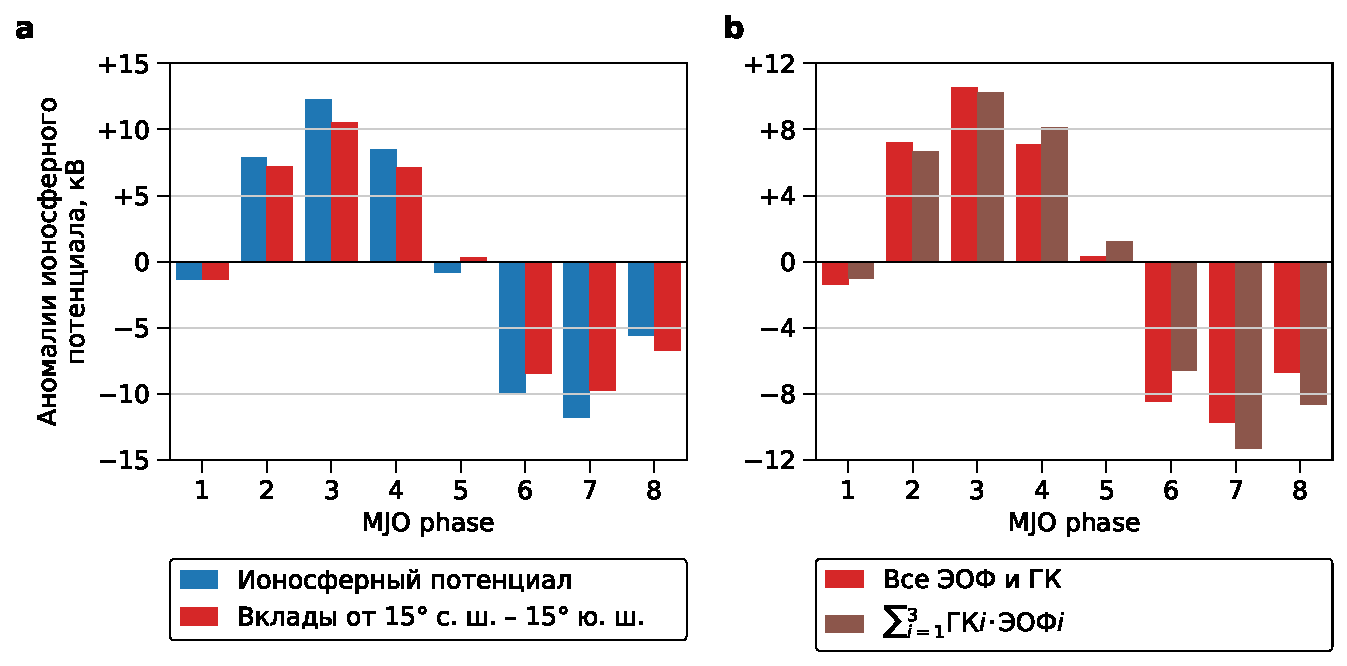
\includegraphics[width=\textwidth]{figures/equatorial_variation.pdf}
    \caption{(a): Аномалии аномалии ИП и вклада в ИП приэкваториального региона (15\textdegree\ с. ш.~--~15\textdegree~ю.~ш.) в различные фазы КМД. Аномалии вычислялись как отклонения от долговременных средних значений. Из вклада приэкваториального региона была убрана изменчивость, имеющая отношение к ЭНЮК и сезонному циклу, как описано в разделе \ref{sec:preliminary_processing}. (b): Аномалии вклада приэкваториального региона в ИП (то же самое, что и на панели (a)) и разложение такой аномалии по первым трём ЭОФ.}
    \label{fig:eq_var}
\end{figure}

\subsubsection{ВЫЧИСЛЕНИЕ ЭОФ И ГК ДЛЯ ВКЛАДОВ В ИП}

После вычитания связей вкладов в ЭНЮК и сезонным циклом получается временной ряд 360-мерных векторов (один вектор для каждого моделируемого дня), содержащих вклады в ИП различных вытянутых вдоль меридиан полос 1\textdegree\texttimes30\textdegree, отвечающих различным долготам. Такой вектор для дня $d$ будет обозначаться через
\begin{equation}
    \vb{V}(d) = \qty(V_1(d),\, \ldots,\, V_{360}(d)).
\end{equation}
Чтобы ЭОФ и ГК были корректно вычислены, требуется перейти к вектору, каждая компонента которого имеет среднее значение, равное нулю. Таким вектором будет 
\begin{equation}
    \vb{U}(d) = \qty(U_1(d),\, \ldots,\, U_{360}(d)),
\end{equation}
где $U_j(d) = V_i(d) - \langle V_i(d) \rangle$ (угловые скобки обозначают долгосрочное усреднение по $d$).

Ниже будет описан процесс вычленения ЭОФ \cite[Гл. 6]{Zhang_Moore_2015} и приведена его имплементация для $\vb{U}(d)$. Можно понимать компоненты данного вектора $U_1(d),\, \ldots,\, U_{360}(d)$ как координаты 360-мерного вектора в стандартном базисе в пространстве $\mathbb{R}^{360}$ $\vb{e}^{(1)},\, \ldots,\, \vb{e}^{(360)}$. Главная идея ЭОФ-анализа заключается в нахождении такого другого ортонормированного базиса $\vb{f}^{(1)},\, \ldots,\, \vb{f}^{(360)}$, что его первые компоненты (то есть  $\vb{f}^{(1)},\, \vb{f}^{(2)}$ и так далее) в некотором смысле описывали наибольшую часть изменчивости $\vb{U}(d)$. Нахождение такого базиса позволит устроить разложение
\begin{equation}
    \label{eq:decomp}
    \vb{U}(d) = \sum\limits_{j=1}^{360} U_j(d) \vb{e}^{(j)} = \sum\limits_{j=1}^{360} C_j(d) \vb{f}^{(j)}.
\end{equation}
Элементы нового базиса $\vb{f}^{(1)},\, \ldots,\, \vb{f}^{(360)}$ называются ЭОФ, а временные коэффициенты разложения по нему $C_1(d),\, \ldots,\, C_{360}(d)$ называются ГК. Стоит заметить, что $\vb{f}^{(j)}$ является 360-мерным вектором и в стандартном базисе $\vb{e}^{(1)},\, \ldots,\, \vb{e}^{(360)}$ записывается в виде
\begin{equation}
    \vb{f}^{(j)} = \qty({f}_1^{(j)},\, \ldots,\, {f}_{360}^{(j)}),
\end{equation}
то есть $\vb{f}^{(j)}$ можно понимать как функцию долготы.

Ниже будет дано строгое математическое определение ЭОФ и ГК, для чего будет использоваться скалярное произведение в пространстве $\mathbb{R}^{360}$, определенное следующим образом:
\begin{equation}
    \qty(\vb{a},\, \vb{b}) = \sum\limits_{j=1}^{360} a_j b_j,\; \text{где}\; \vb{a} = \sum\limits_{j=1}^{360} a_j \vb{e}^{(j)},\; \vb{b} = \sum\limits_{j=1}^{360} b_j \vb{e}^{(j)}.
\end{equation}
Под нормой будет пониматься 
\begin{equation}
    \norm{\vb{a}} = \sqrt{\sum\limits_{j=1}^{360} a_j},\; \text{где}\; \vb{a} = \sum\limits_{j=1}^{360} a_j \vb{e}^{(j)}.
\end{equation}
То есть будут использоваться стандартное скалярное произведение в пространстве $\mathbb{R}^{360}$ и стандартная евклидова норма. Первая ЭОФ $\vb{f}^{(1)}$ определяется как такое единичный вектор ($\norm{\vb{f}^{(1)}}=1$), который минимизирует величину
\begin{equation}
    \epsilon_1 = \expval{\norm{\vb{U}(d) - (\vb{U}(d),\, \vb{f}^{(1)})\vb{f}^{(1)}}^2}.
\end{equation}
Похожим образом определяется вторая ЭОФ $\vb{f}^{(2)}$. Согласно определению $\vb{f}^{(2)}$ есть такой единичный вектор ($\norm{\vb{f}^{(2)}}=1$) ортогональный $\vb{f}^{(1)}$ ($\qty(\vb{f}^{(1)},\, \vb{f}^{(2)})=0$), который минимизирует величину
\begin{equation}
    \epsilon_2 = \expval{\norm{\vb{U}(d) - (\vb{U}(d),\, \vb{f}^{(1)})\vb{f}^{(1)} - (\vb{U}(d),\, \vb{f}^{(2)})\vb{f}^{(2)}}^2}.
\end{equation}
Следующие ЭОФ определяются аналогичным образом. То есть, например, $j$-ая ЭОФ $\vb{f}^{(j)}$ есть такой единичный вектор ($\norm{\vb{f}^{(j)}}=1$) ортогональный $\vb{f}^{(1)},\, \ldots,\, \vb{f}^{(j-1)}$, который минимизирует величину
\begin{equation}
    \epsilon_j = \expval{\norm{\vb{U}(d) - \sum\limits_{k=1}^{j} \qty(\vb{U}(d),\, \vb{f}^{(k)})\vb{f}^{(k)}}^2}.
\end{equation}
ГК определяются как координаты $\vb{U}(d)$ в новом базисе. Например, $j$-ая ГК $C_j(d)$ задаётся формулой
\begin{equation}
    C_j(d) = (\vb{U}(d),\, \vb{f}^{(j)}).
    \label{eq:pc}
\end{equation}

Можно придать ЭОФ более наглядный смысл. Пользуясь тем, что $\expval{U_j(d)}=0$ для всех $j$, не трудно показать, что
\begin{equation}
    \epsilon_1 = \expval{\norm{\vb{U}(d)}^2} - \expval{\qty(\vb{U}(d),\, \vb{f}^{(1)})^2} = \sum\limits_{j=1}^{360} \mathrm{Var}\, U_j(d) - \mathrm{Var}\, C_1(d),
\end{equation}
где через $\mathrm{Var}$ обозначена дисперсия. Аналогично можно получить
\begin{equation}
    \epsilon_j = \expval{\norm{\vb{U}(d)}^2} - \sum\limits_{k=1}^{j} \expval{\qty(\vb{U}(d),\, \vb{f}^{(k)})^2} = \sum\limits_{j=1}^{360} \mathrm{Var}\, U_j(d) - \sum\limits_{k=1}^{j}\mathrm{Var}\, C_j(d).
\end{equation}
Отсюда видно, что первая ЭОФ $\vb{f}^{(1)}$ максимизирует $\mathrm{Var}\, C_1(d)$, вторая ЭОФ $\vb{f}^{(2)}$ выбирается в оставшихся измерениях таким образом, чтобы максимизировать $\mathrm{Var}\, C_2(d)$ и так далее.

Численное нахождение ЭОФ основано на поиске собственных векторов и собственных значений ковариационной матрицы $\Sigma$, элементы которой определяются как
\begin{equation}
    \Sigma_{ij} = \mathrm{Cov}\, \qty(U_i(d), U_j(d)).
\end{equation}
Можно показать, что ковариационная матрица является симметричной и положительно определенной \cite[Утв. 6.1]{Zhang_Moore_2015}, отсюда следует, что собственные значения такой матрицы будут действительными положительными числами. Нетрудно показать, что первая ЭОФ является собственным вектором матрицы $\Sigma$, отвечающим наибольшему собственному значению, вторая ЭОФ является собственным вектором матрицы $\Sigma$, отвечающим второму по величине собственному значению и так далее \cite[Tеор. 6.1 и 6.3]{Zhang_Moore_2015}. После нахождения ЭОФ по формуле \eqref{eq:pc} находят ГК.

Принято вводить такую величину, как объясняемая дисперсия. Она определяется для каждой из ЭОФ и в некотором смысле показывает какую часть дисперсии объясняет данная ЭОФ. Если говорить строго, что объясняемая дисперсия $j$-ой ЭОФ определяется как $\mathrm{Var}\, C_j(d)$. Можно доказать, что объясняемая дисперсия $j$-ой ЭОФ равна $j$-ому собственному значению ковариационной матрицы $\Sigma$ \cite[Утв. 6.2]{Zhang_Moore_2015}.

Таким образом, переход к базису, образованному из ЭОФ, позволяет устроить разложение \eqref{eq:decomp}, то есть представить вектор $\vb{U}(d)$ в виде суммы взаимно ортогональных компонент $C_1(d)\vb{f}^{(1)},\, \ldots,\, C_{360}(d) \vb{f}^{(360)}$, первые несколько из которых отвечают за наибольшую часть дисперсии данных.

Основываясь на \eqref{eq:decomp} можно записать аномалию суммарного вклада в ИП от приэкваториального региона (без изменчивости, связанной с ЭНЮК и сезонным циклом) за день $d$ в виде
\begin{equation}
\label{eq:u_eq}
    U_{\mathrm{eq}} (d) = \sum\limits_{j=1}^{360} U_j(d) = \sum\limits_{j,i=1}^{360} C_i(d) f_j^{(i)}.
\end{equation}
Если же вместо вектора $\vb{U}(d)$ перейти к рассмотрению его главной части, которая согласно смыслу ЭОФ, описывается первыми несколькими ЭОФ, то есть к вектору
\begin{equation}
\label{eq:u_tilde}
    \Tilde{\vb{U}}(d) = C_1(d) \vb{f}^{(1)} + C_2(d) \vb{f}^{(2)} + C_3(d) \vb{f}^{(3)},
\end{equation}
где учтены лишь первые три ЭОФ, то соответствующая такому вектору аномалия вклада будет даваться выражением
\begin{equation}
\label{eq:u_tilde_eq}
    \Tilde{U}_{\mathrm{eq}}(d) =\sum\limits_{j=1}^{360} \qty{C_1(d) {f}_j^{(1)} + C_2(d) {f}_j^{(2)} + C_3(d) {f}_j^{(3)}} = \sum\limits_{j=1}^{360} \sum\limits_{i=1}^{3} C_i(d) f_j^{(i)}.
\end{equation}
На рис. \ref{fig:eq_var}{b} проводится сравнение средних значений $U_{\mathrm{eq}} (d)$ и $\Tilde{U}_{\mathrm{eq}}(d)$ в различные фазы КМД. Видно, что для воспроизведения синусоидальной вариации, которая присутствует во всей сумме, хватает учёта лишь первых трёх ЭОФ. Это позволяет рассматривать \eqref{eq:u_tilde} и \eqref{eq:u_tilde_eq} вместо \eqref{eq:decomp} и \eqref{eq:u_eq} с целью исследования физического механизма, лежащего за наблюдаемой вариацией.

Чтобы исследовать более детально вариацию $\Tilde{U}_{\mathrm{eq}}(d)$ на масштабе КМД, представленную на рис. \ref{fig:eq_var}{b}, следует разложить такую вариацию на раздельные части, отвечающие различным ЭОФ. Рис. \ref{fig:eofs_and_pcs}{a} показывает каждое из трёх слагаемых \eqref{eq:u_tilde}, усреднённое по различным фазам КМД. Вклад в ИП, отвечающий ЭОФ1, равен
\begin{equation}
\label{eq:u1}
    U_\mathrm{eq}^{(1)} (d) = C_1(d) \sum\limits_{j=1}^{360} {f}_j^{(1)}
\end{equation}
и имеет на масштабе КМД синусоидальную вариацию с максимумом в четвертой фазе и минимумом в 8 фазе. Вклады в ИП, отвечающие ЭОФ2 и ЭОФ3, равны
\begin{equation}
\label{eq:u23}
    \begin{split}
        U_\mathrm{eq}^{(2)} (d) = C_2(d) \sum\limits_{j=1}^{360} {f}_j^{(2)},\\
        U_\mathrm{eq}^{(3)} (d) = C_3(d) \sum\limits_{j=1}^{360} {f}_j^{(3)}
    \end{split}
\end{equation}
и имеют близкие синусоидальные вариации на масштабе КМД с максимумом во второй фазе и минимумом в шестой.

\begin{figure}[htbp]
    \centering
    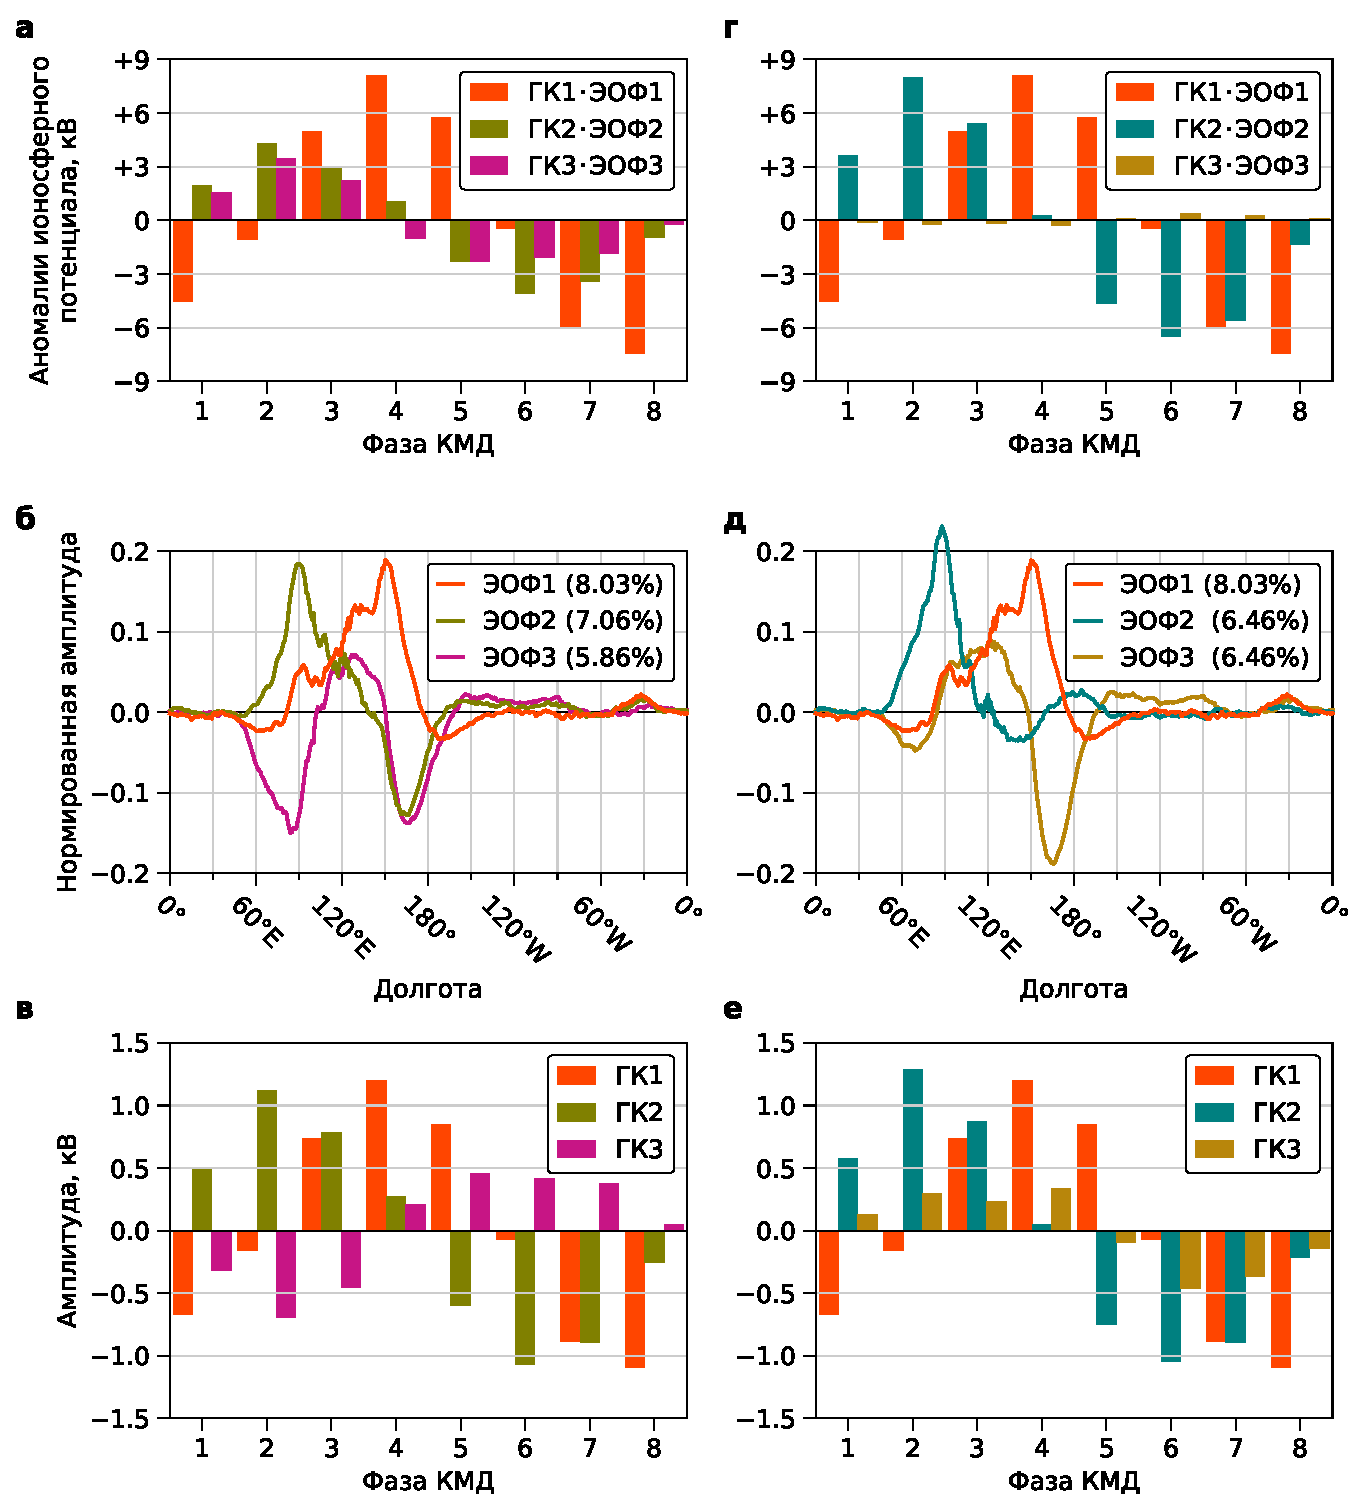
\includegraphics[width=\textwidth]{figures/eofs_and_pcs.pdf}
    \caption{(a): Изменчивость вклада в ИП экваториального региона (15\textdegree\ с. ш.~--~15\textdegree~ю.~ш.) в различные фазы КМД, отвечающая каждой из первых трёх ЭОФ в отдельности. (b): Пространственная структура первых трёх ЭОФ. (c): ГК, отвечающие первым трём ЭОФ, усреднённые за различные фазы КМД. (d)--(f): То же, что и (a)--(c) для повернутых ЭОФ. Числа в легендах графиков панелей (b) и (e) обозначают объясняемую дисперсию данной ЭОФ.}
    \label{fig:eofs_and_pcs}
\end{figure}

Рис. \ref{fig:eofs_and_pcs}{b} демонстрирует долготные профили первых трёх ЭОФ (ЭОФ1 $\vb{f}^{(1)}$, ЭОФ2 $\vb{f}^{(2)}$ и ЭОФ3 $\vb{f}^{(3)}$). ЭОФ1 описывает значительную аномалию во вкладах в ИП, расположенную между долготами 80\textdegree\ в. д. и 180\textdegree и имеющую максимум на 150\textdegree\ в. д.. ЭОФ2 и ЭОФ3 больше всего отличны от нуля между 50\textdegree\ в. д. и 170\textdegree\ з. д., они обе имеют сильный минимум между 160\textdegree\ в. д. и 170\textdegree\ в. д., кроме того около 90\textdegree\ з. д. они достигают экстремумов противоположного знака.

С целью большей наглядности на рис. \ref{fig:eofs_and_pcs}{c} приведены усреднённые по различным фазам КМД ГК, отвечающие первым трём ЭОФ (то есть ГК1 $C_1(d)$, ГК2 $C_2(d)$ и ГК3 $C_3(d)$). Важно понимать, что усреднённые ГК пропорциональны усреднённым аномалиям вкладам в ИП, отвечающим различным ЭОФ, (см. рис. \ref{fig:eofs_and_pcs}{a}), это прямо следует из выражений \eqref{eq:u1} и \eqref{eq:u23}, а так же того факта, что ЭОФ лишь описывают пространственную структуру вкладов и не меняются со временем.

\subsubsection{ПОВОРОТ БАЗИСА ЭОФ}
\label{sec:rot_eof}

Из рис. \ref{fig:eofs_and_pcs}{c} видно, что ГК2 и ГК3 изменяются на масштабе КМД в противофазе. В то же время соответствующие им ЭОФ, ЭОФ2 и ЭОФ3, как функции долготы крайне схожи на востоке около 150\textdegree\ в. д., но сильно расходятся около 90\textdegree\ в. д. (см. рис. \ref{fig:eofs_and_pcs}{b}). Это наводит на мысль о возможности введения более простых пространственных паттернов; вместо ЭОФ2 $\vb{f}^{(2)}$ и ЭОФ3 $\vb{f}^{(3)}$ можно перейти к
\begin{equation}
    \vb{f}^{(2')} = \dfrac{\vb{f}^{(2)} - \vb{f}^{(3)}}{\sqrt{2}},\; \vb{f}^{(3')} = \dfrac{\vb{f}^{(2)} + \vb{f}^{(3)}}{\sqrt{2}},
\end{equation}
которые будут обозначаться через ЭОФ2' и ЭОФ3' соответственно. Аналогично, вместо ГК2 $C_2(d)$ и ГК3 $C_3(d)$ следует перейти к 
\begin{equation}
    C_{2'}(d) = \dfrac{C_2(d) - C_3(d)}{\sqrt{2}} ,\;  C_{3'}(d)  = \dfrac{C_2(d) + C_3(d)}{\sqrt{2}},
\end{equation}
которые будут обозначаться через ГК2' и ГК3'. Такая техника называется поворотом ЭОФ \cite[Гл. 6]{Zhang_Moore_2015}, грубо говоря, данная техника позволяет подогнать автоматически выбранный базис к решаемой проблеме (стоит заметить, что оригинальные ЭОФ были рассчитаны без каких-либо предположений о КМД, его временных и пространственных масштабов).

В повернутом базисе ЭОФ выражения \eqref{eq:u_tilde} и \eqref{eq:u_tilde_eq} примут вид
\begin{equation}
    \Tilde{\vb{U}}(d) = C_1(d) \vb{f}^{(1)} + C_{2'}(d) \vb{f}^{(2')} + C_{3'}(d) \vb{f}^{(3')},
\end{equation}
\begin{equation}
\label{eq:u_tilde_eq_new}
    \Tilde{U}_{\mathrm{eq}}(d) =\sum\limits_{j=1}^{360} \qty{C_1(d) {f}_j^{(1)} + C_{2'}(d) {f}_j^{(2')} + C_{3'}(d) {f}_j^{(3')}},
\end{equation}
выражение \eqref{eq:u1} останется прежним, вместо выражения \eqref{eq:u23} следует использовать
\begin{equation}
    \begin{split}
        U_\mathrm{eq}^{(2')} (d) = C_{2'}(d) \sum\limits_{j=1}^{360} {f}_j^{(2')},\\
        U_\mathrm{eq}^{(3')} (d) = C_{3'}(d) \sum\limits_{j=1}^{360} {f}_j^{(3')}.
    \end{split}
\end{equation}

Рис. \ref{fig:eofs_and_pcs}{e} и рис. \ref{fig:eofs_and_pcs}{f} являются аналогами рис. \ref{fig:eofs_and_pcs}{b} и рис. \ref{fig:eofs_and_pcs}{c} для повернутых ЭОФ (ЭОФ1 $\vb{f}^{(1)}$, ЭОФ2' $\vb{f}^{(2')}$ и ЭОФ3' $\vb{f}^{(3')}$) и новых ГК (ГК1 $C_1(d)$, ГК2' $C_{2'}(d)$ и ГК3' $C_{3'}(d)$). Из сравнения рис. \ref{fig:eofs_and_pcs}{e}  с \ref{fig:eofs_and_pcs}{b} видно, что пространственная структура новых ЭОФ стала действительно проще по сравнению со структурой оригинальных ЭОФ. ЭОФ2' описывает в значительной степени аномалию вкладов в ИП, расположенных между 50\textdegree\ в. д. и 120\textdegree\ в. д. с одним крупным максимумом в районе 90\textdegree\ в. д., в то время как ЭОФ3' описывает более сложную структуру вкладов с главным экстремумов в районе 170\textdegree\ в. д.. Если посмотреть на средние значения ГК в течение фаз КМД (см. рис. \ref{fig:eofs_and_pcs}{f}), то видно, что в среднем значения ГК3' меньше по абсолютной величине, чем значения ГК2' и ГК1. Поэтому в дальнейшем можно удержать лишь ЭОФ1 и ЭОФ2', пренебрегая ЭОФ3'.

Далее следует рассмотреть аномалии вклада экваториального региона в ИП. Рис. \ref{fig:eofs_and_pcs}{d} демонстрирует три слагаемых разложения \eqref{eq:u_tilde_eq_new}, усреднённых по различным фазам КМД (аналогично рис. \ref{fig:eofs_and_pcs}{a}, где были изображены слагаемые разложения \eqref{eq:u_tilde_eq}). Легко видеть, что слагаемое $U_\mathrm{eq}^{(3')} (d)$, относящееся к ЭОФ3', пренебрежимо мало, что не удивительно, ведь не только ГК3' мала по сравнению с двумя прочими ГК, но и сумма компонент ЭОФ3' $\sum_{j=1}^{360} {f}_j^{(3')}$ мала (см. кривую ЭОФ3' на рис. \ref{fig:eofs_and_pcs}{e}). Остальные слагаемые $U_\mathrm{eq}^{(1)} (d)$ и $U_\mathrm{eq}^{(2')} (d)$, отвечающие ЭОФ1 и ЭОФ2' соответственно, имеют синусоидальные вариации по фазам КМД с близкими амплитудами. Одна вариация обгоняет другую на 1 четверть периода (2 фазы КМД). Вариация аномалии ИП, показанная на рис. \ref{fig:eq_var}, может быть во многом приближена суммой двух таких базовых колебаний.

\subsubsection{ДОЛГОТНАЯ СТРУКТУРА БАЗОВЫХ КОЛЕБАНИЙ}

Таким образом поворот базиса, составленного из ЭОФ, позволил свести наблюдаемую вариацию ИП по фазам КМД (см. рис. \ref{fig:variations}{a}) к суперпозиции двух базовых колебаний, задаваемых усредненными $U_\mathrm{eq}^{(1)} (d)$ и $U_\mathrm{eq}^{(2')} (d)$ по фазам КМД (см. рис. \ref{fig:eofs_and_pcs}{d}). Если рассуждать в терминах пространственных паттернов, то величины $U_\mathrm{eq}^{(1)} (d)$ и $U_\mathrm{eq}^{(2')} (d)$ определяются как суммы компонент векторов
\begin{equation}
    \vb{U}^{(1)}(d) = C_1(d) \vb{f}^{(1)}
    \label{eq:u_eof1}
\end{equation}
и
\begin{equation}
    \vb{U}^{(2')}(d) = C_{2'}(d) \vb{f}^{(2')}
    \label{eq:u_eof2'}
\end{equation}
вдоль долготных индексов. В данном разделе будет рассмотрена долготная структура данных векторов в различные фазы КМД (то есть суммирование по долготным индексам проводиться не будет).

Левый столбец рис. \ref{fig:longitudinal_structure} показывает усредненную долготную структуру аномалий экваториальных вкладов в ИП (то есть $\vb{U}(d)$ из выражения \eqref{eq:decomp}) для различных фаз КМД. Это буквально одномерная версия рис. \ref
{fig:map_of_contributions}: аномалии вкладов клеток 1\textdegree\texttimes1\textdegree в ИП, показанные на рис. \ref{fig:map_of_contributions}, составляют аномалии вкладов от вытянутых вдоль меридиан полос 1\textdegree\texttimes30\textdegree, показанные в левом столбце рис. \ref{fig:longitudinal_structure}; именно поэтому красные и синие области на рис. \ref{fig:map_of_contributions}, обозначающие положительные и отрицательные аномалии вкладов соответственно, в основном совпадают с интервалами положительных и отрицательных аномалий в левом столбце рис. \ref{fig:longitudinal_structure}.

\begin{figure}[htbp]
    \centering
    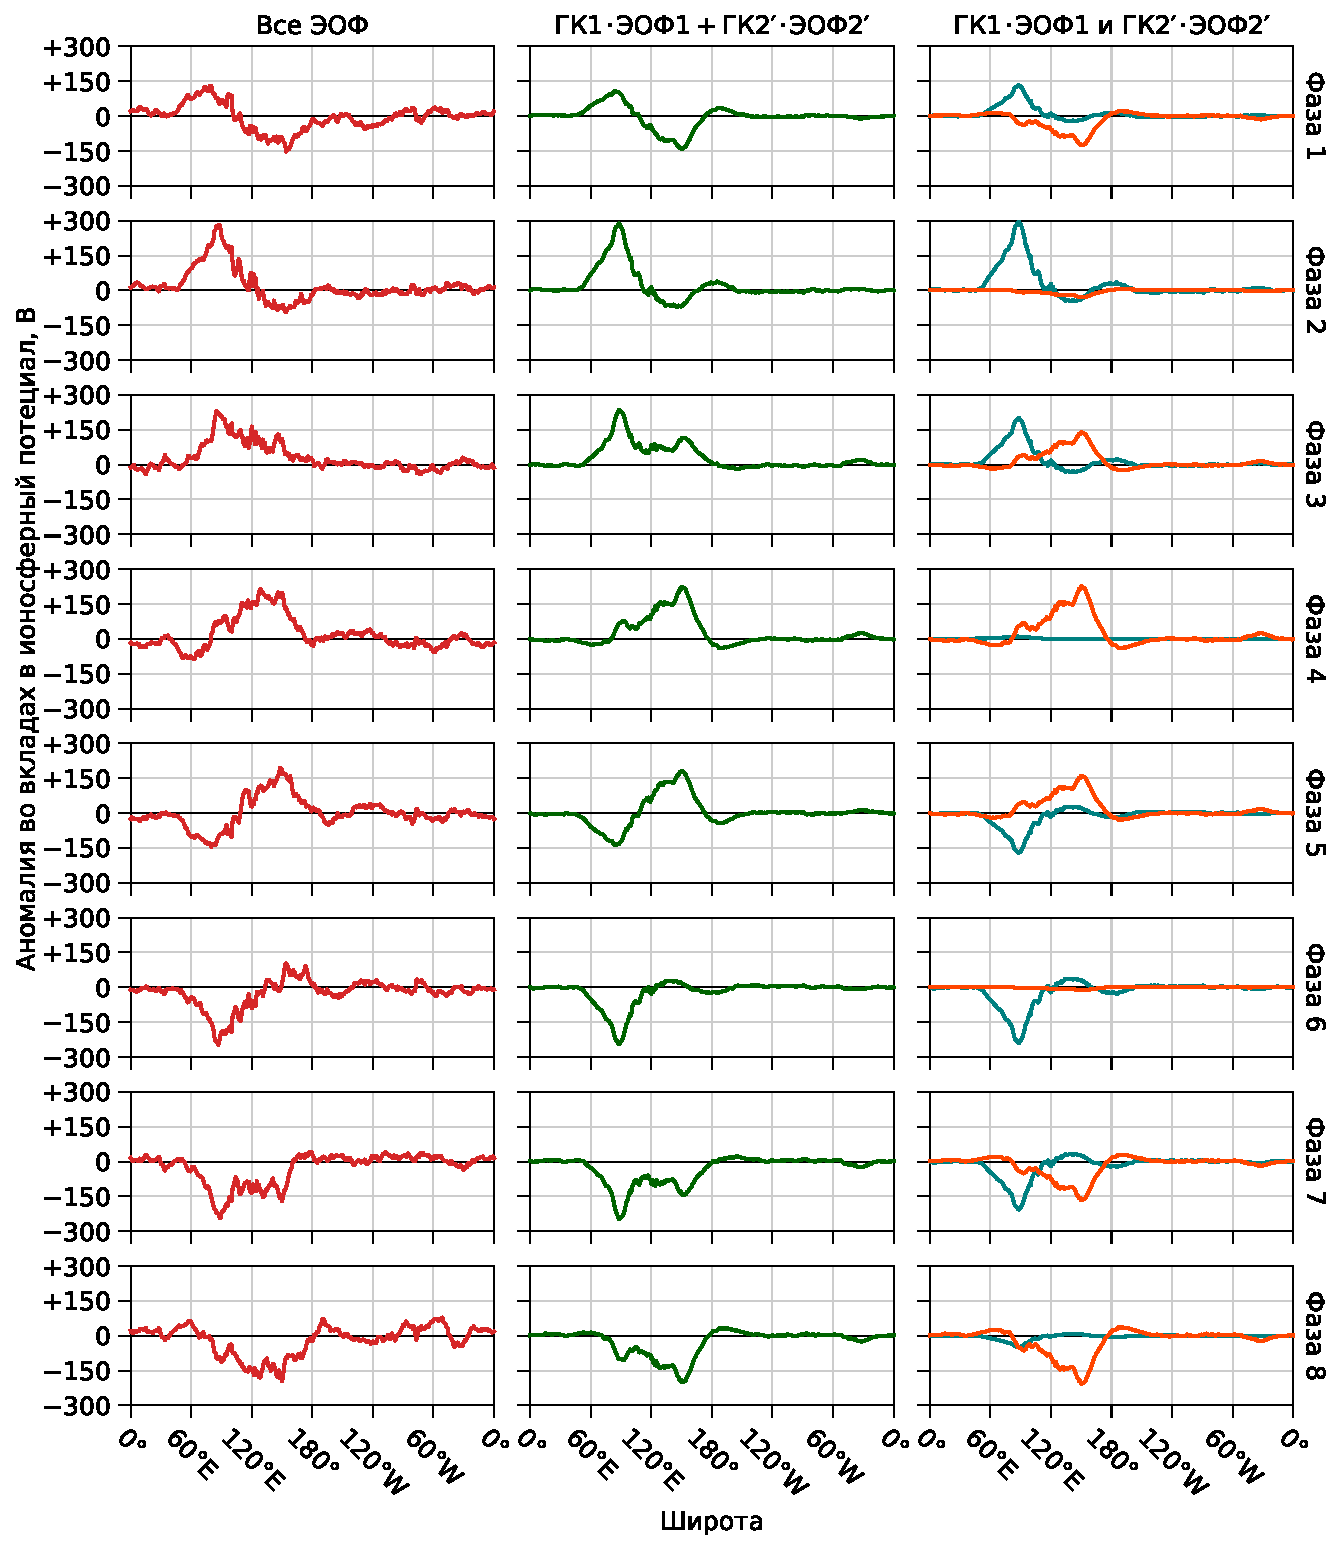
\includegraphics[width=\textwidth]{figures/longitudinal_structure.pdf}
    \caption{Левый столбец: Аномалии вкладов в ИП от вытянутых вдоль меридиан полос 1\textdegree\texttimes30\textdegree\ (15\textdegree\ с. ш.~--~15\textdegree\ ю. ш.) при различных долготах в течение каждой из восьми фаз КМД. Аномалии вычисляются по отношении к долгосрочным средним значениям. Изменчивость, связанная с ЭНЮК и сезонным циклом, удалена из данных (см. раздел \ref{sec:preliminary_processing}) перед построением графиков. Средний столбец: то же самое за тем исключением, что была оставлена лишь изменчивость, относящаяся к ЭОФ1 и ЭОФ2' (см. раздел \ref{sec:rot_eof}). Правый столбец: Изменчивость, отвечающая ЭОФ1 и ЭОФ2', показана раздельно.}
    \label{fig:longitudinal_structure}
\end{figure}

Средний столбец рис. \ref{fig:longitudinal_structure} показывает левый столбец преобразуется, если вместо разложения по всем ЭОФ, которое может быть записано как
\begin{equation}
    \vb{U}(d) = C_1(d) \vb{f}^{(1)} + C_{2'}(d) \vb{f}^{(2')} + C_{3'}(d) \vb{f}^{(3')} + \sum\limits_{j=4}^{360} C_j(d) \vb{f}^{j},
\end{equation}
удержать лишь первые два слагаемых. Сравнивая средний и левый столбцы, можно заключить, что учёт лишь слагаемых, отвечающих ЭОФ1 и ЭОФ2', сохраняет главные паттерны в динамики вкладов в ИП на масштабах КМД.

Правый столбце рис. \ref{fig:longitudinal_structure} разлагает то, что было показано в среднем столбце, на две компоненты, показывая раздельно усреднённые аномалии вкладов, отвечающие ЭОФ1 и ЭОФ2'. Можно видеть, что сложная динамика вкладов, наблюдаемая в среднем столбце, оказывается суперпозицией двух простых колебаний, долготная структура которых постоянная и задаётся ЭОФ1 и ЭОФ2' (см. рис. \ref{fig:eofs_and_pcs}{e}). Амплитуда двух выделенных в правом столбце рис. \ref{fig:longitudinal_structure} колебаний имеет синусоидальную вариацию по фазам КМД и определяется ГК1 и ГК2' (см. рис. \ref{fig:eofs_and_pcs}{f}).

Таким образом, компонента \eqref{eq:u_eof1}, отвечающая ЭОФ1, в основном локализована между 80\textdegree\ в. д. и 180\textdegree\ с максимумом на долготе 150\textdegree\ в. д., такая структура в среднем периодичным образом меняется на масштабе КМД, достигая наибольшего значения амплитуды в четвертой фазе и минимального значения амплитуды в восьмой фазе. Компонента \eqref{eq:u_eof2'}, отвечающая ЭОФ2', сконцентрирована между 50\textdegree\ в. д. и 120\textdegree\ в. д. и имеет основной максимум на долготе около 90\textdegree в. д., в среднем такая структура имеет максимум амплитуды во второй фазе КМД и минимум в шестой фазе.

\subsubsection{СВЯЗЬ МЕЖДУ ИП И КМД}

Подводя итог вышеописанному, важно отметить, что удалось выделить два базовых колебания вкладов в ИП на масштабе КМД (см. правый столбец рис. \ref{fig:longitudinal_structure}), одно из которых происходит над Морским континентом (80\textdegree\ в. д. -- 180\textdegree), а второе --- над Индийским океаном (50\textdegree\ в. д. -- 120\textdegree\ в. д.). Второе колебание опережает первое на четверть периода, то есть на 2 фазы КМД; при суммировании вкладов, относящихся к различным долготам, эти два колебания достигают одинаковой амплитуды (см. рис. \ref{fig:eofs_and_pcs}{d}) и вме{}сте дают похожую на синус вариацию с максимумом в третьей фазе и минимумом в седьмой. Это объясняет большую часть изменчивости ИП на масштабе КМД (см. рис. \ref{fig:eq_var}) и таким образом редуцирует задачу объяснения наблюдаемой вариации ИП по фазам КМД (см. рис. \ref{fig:variations}{a}) к пониманию физической природы вышеупомянутой пары базовых колебаний.

Следует напомнить, что двумерный индекс RMM, который используется для численного описания КМД и на основе которого выделяются 8 фаз КМД, был введён в работе \cite